\section*{Problema 3.1}

\textbf{Trabajamos con los de datos fashion MNIST. Se trata de imágenes 28x28 de diez diferentes tipos de prendas. Trabajaremos con \file{fashion-mnist\_train.csv}.  Ver \url{https://www.kaggle.com/zalando-research/fashionmnist}}

\begin{figure}[H]
    \centering
    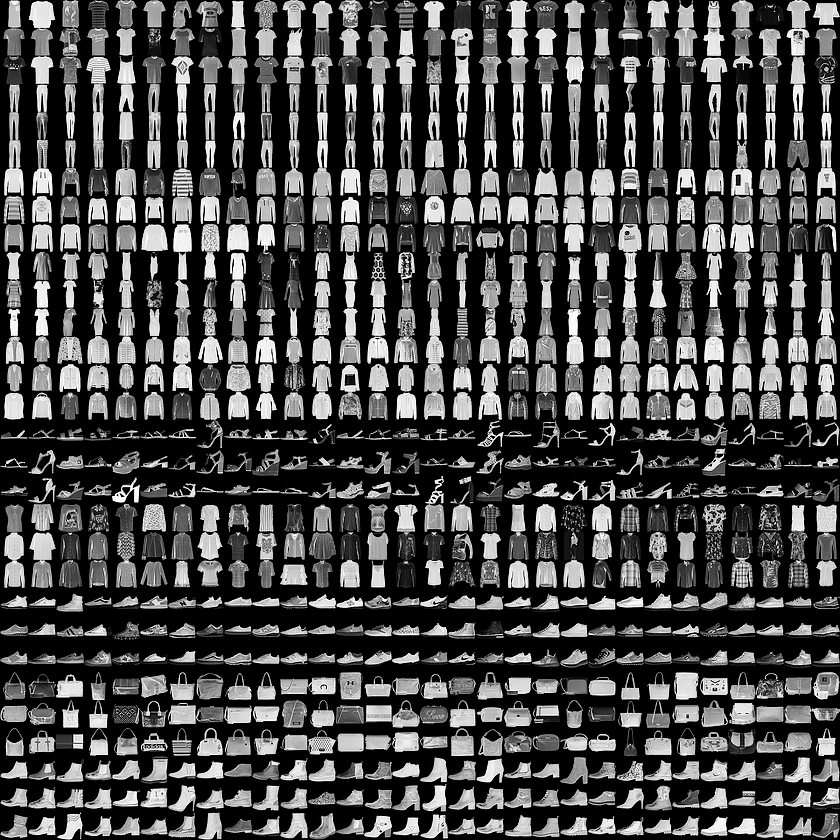
\includegraphics[width=8cm]{Graphics/Problema_3_1.png}
    \caption{}
\end{figure}

\textbf{Busca visualizaciones 2D y 3D basadas en PCA de las imágenes de T-shirts (clase "0`'). ¿ Ves posible encontrar interpretaciones de los componentes como lo hicimos en clase con la base mnist (clásico) de dígitos?}


\subsection*{Visualizaciones 2D}

\begin{figure}[H]
    \centering
    \begin{subfigure}{9.5cm}
        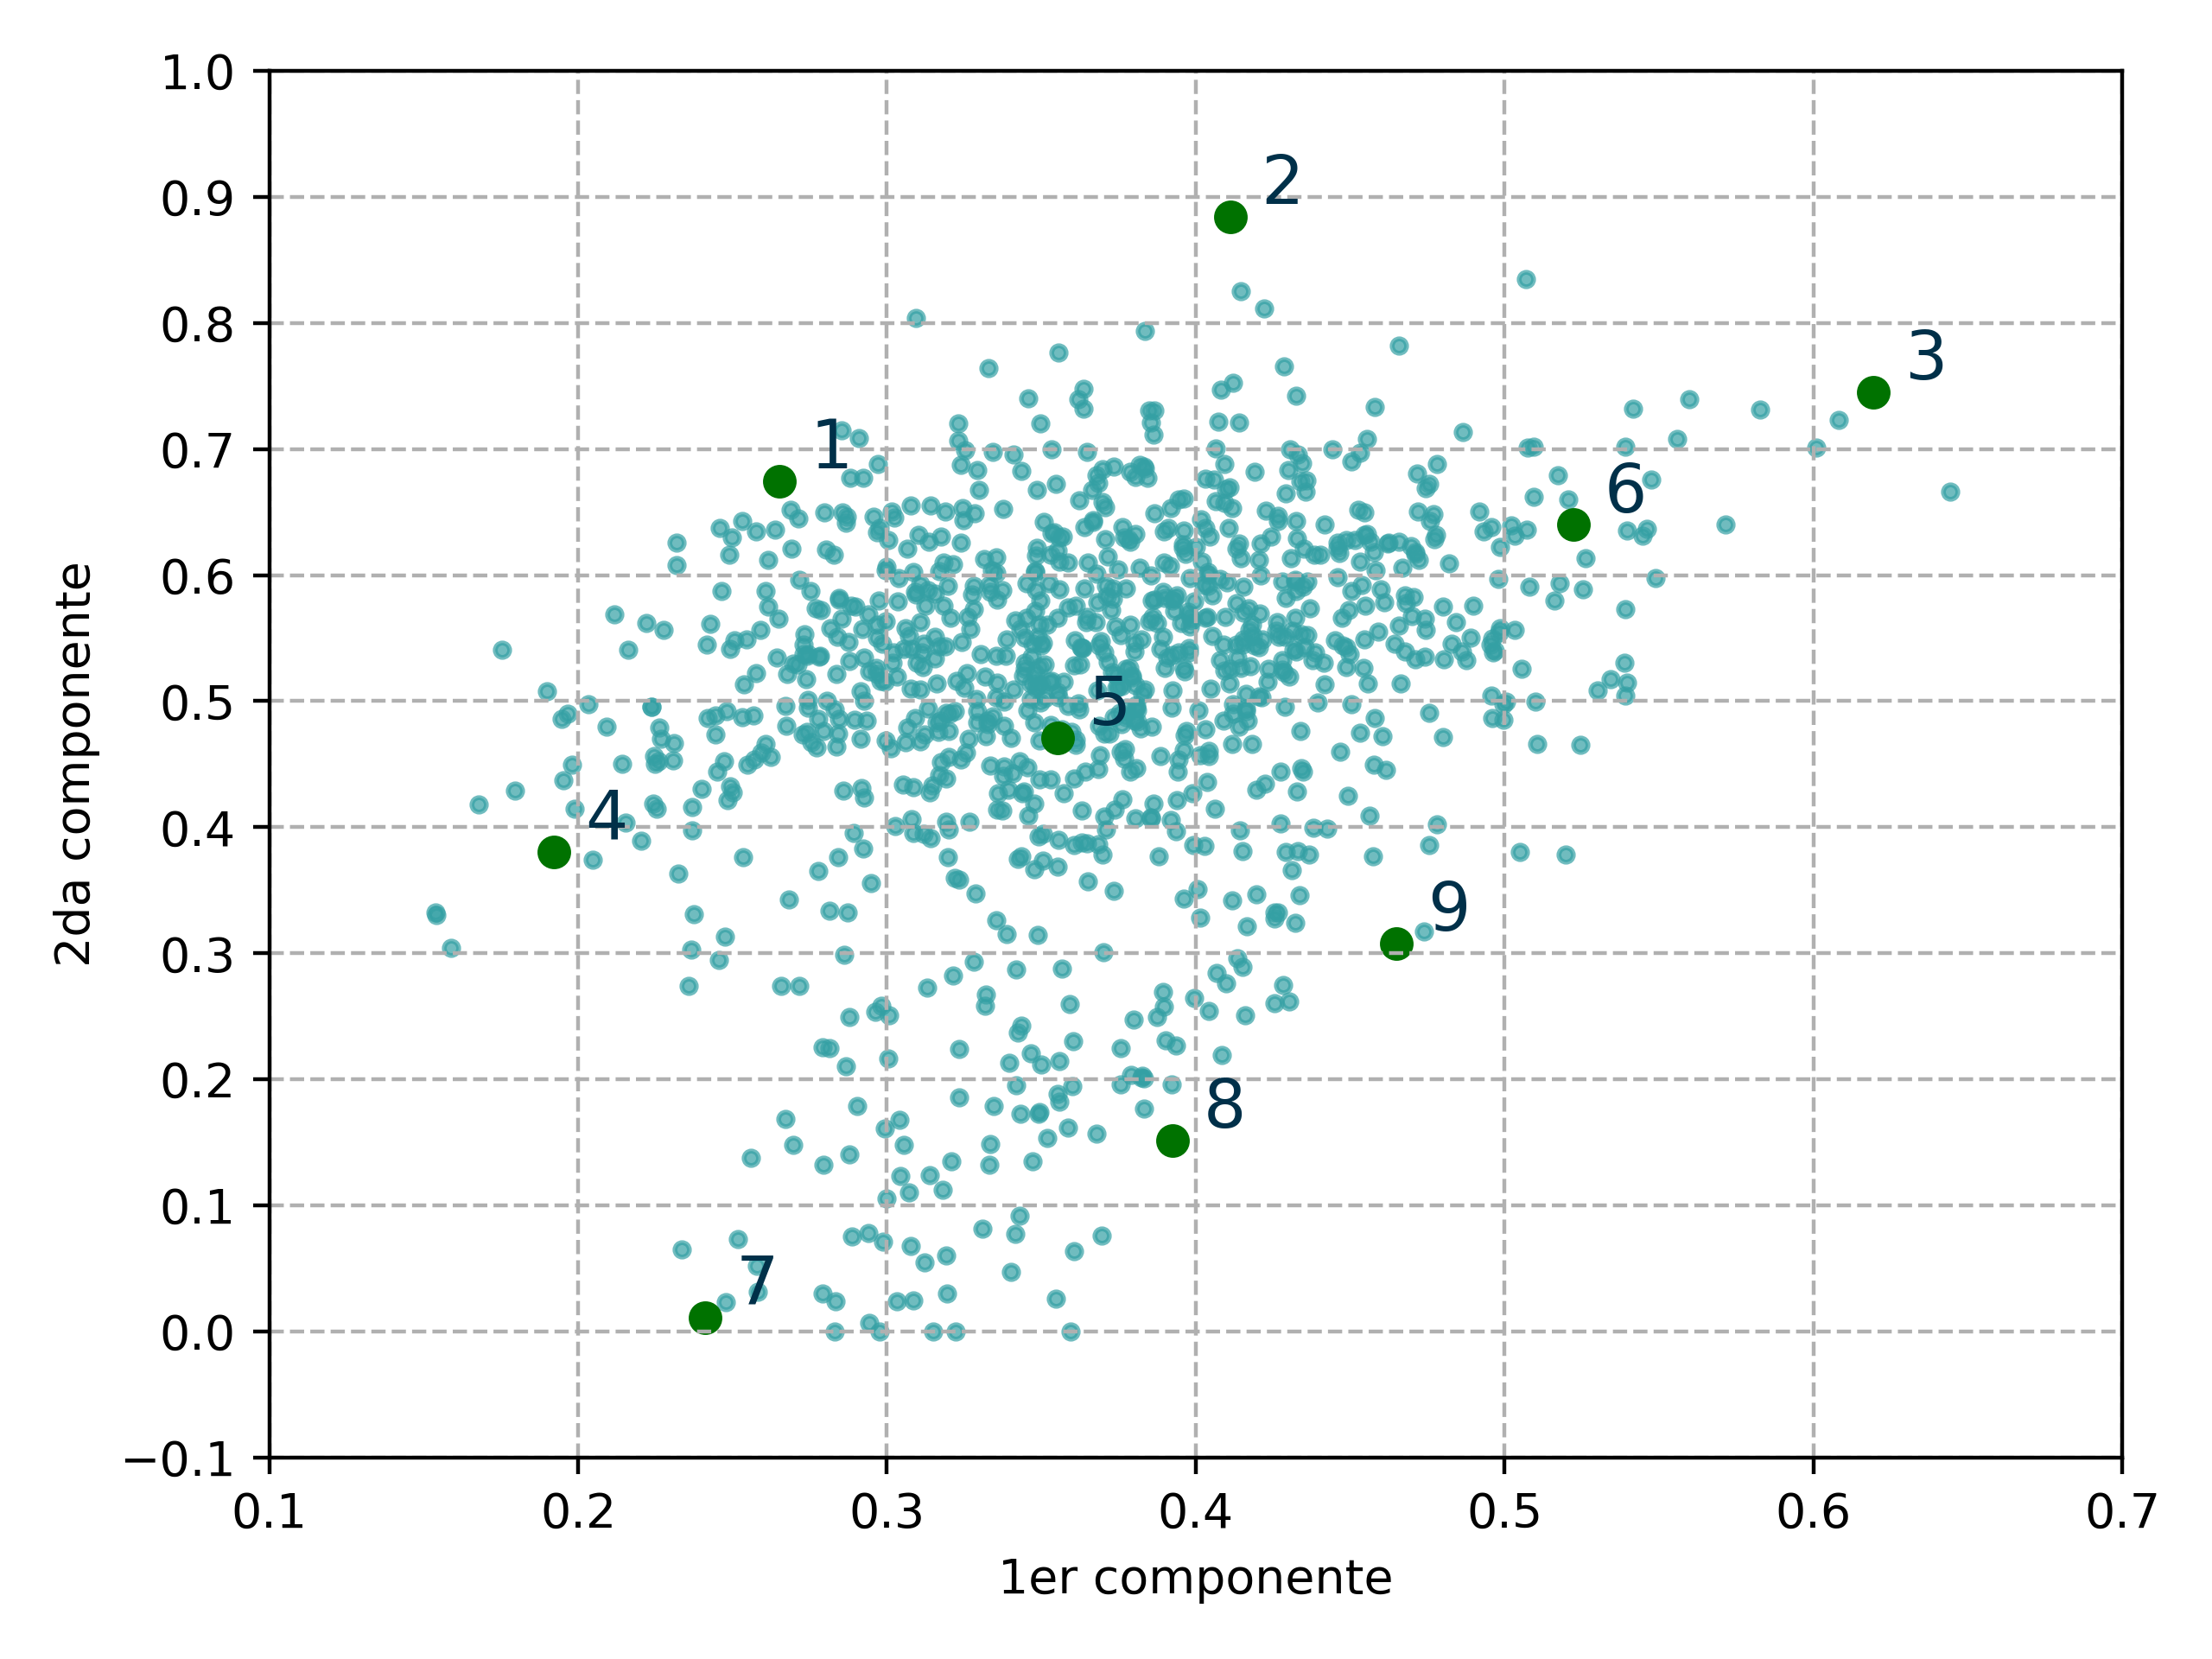
\includegraphics[width=9.5cm]{Graphics/Problema_3_1/loadings_2d.png}
        \caption{}
    \end{subfigure}
    \begin{subfigure}{7cm}
        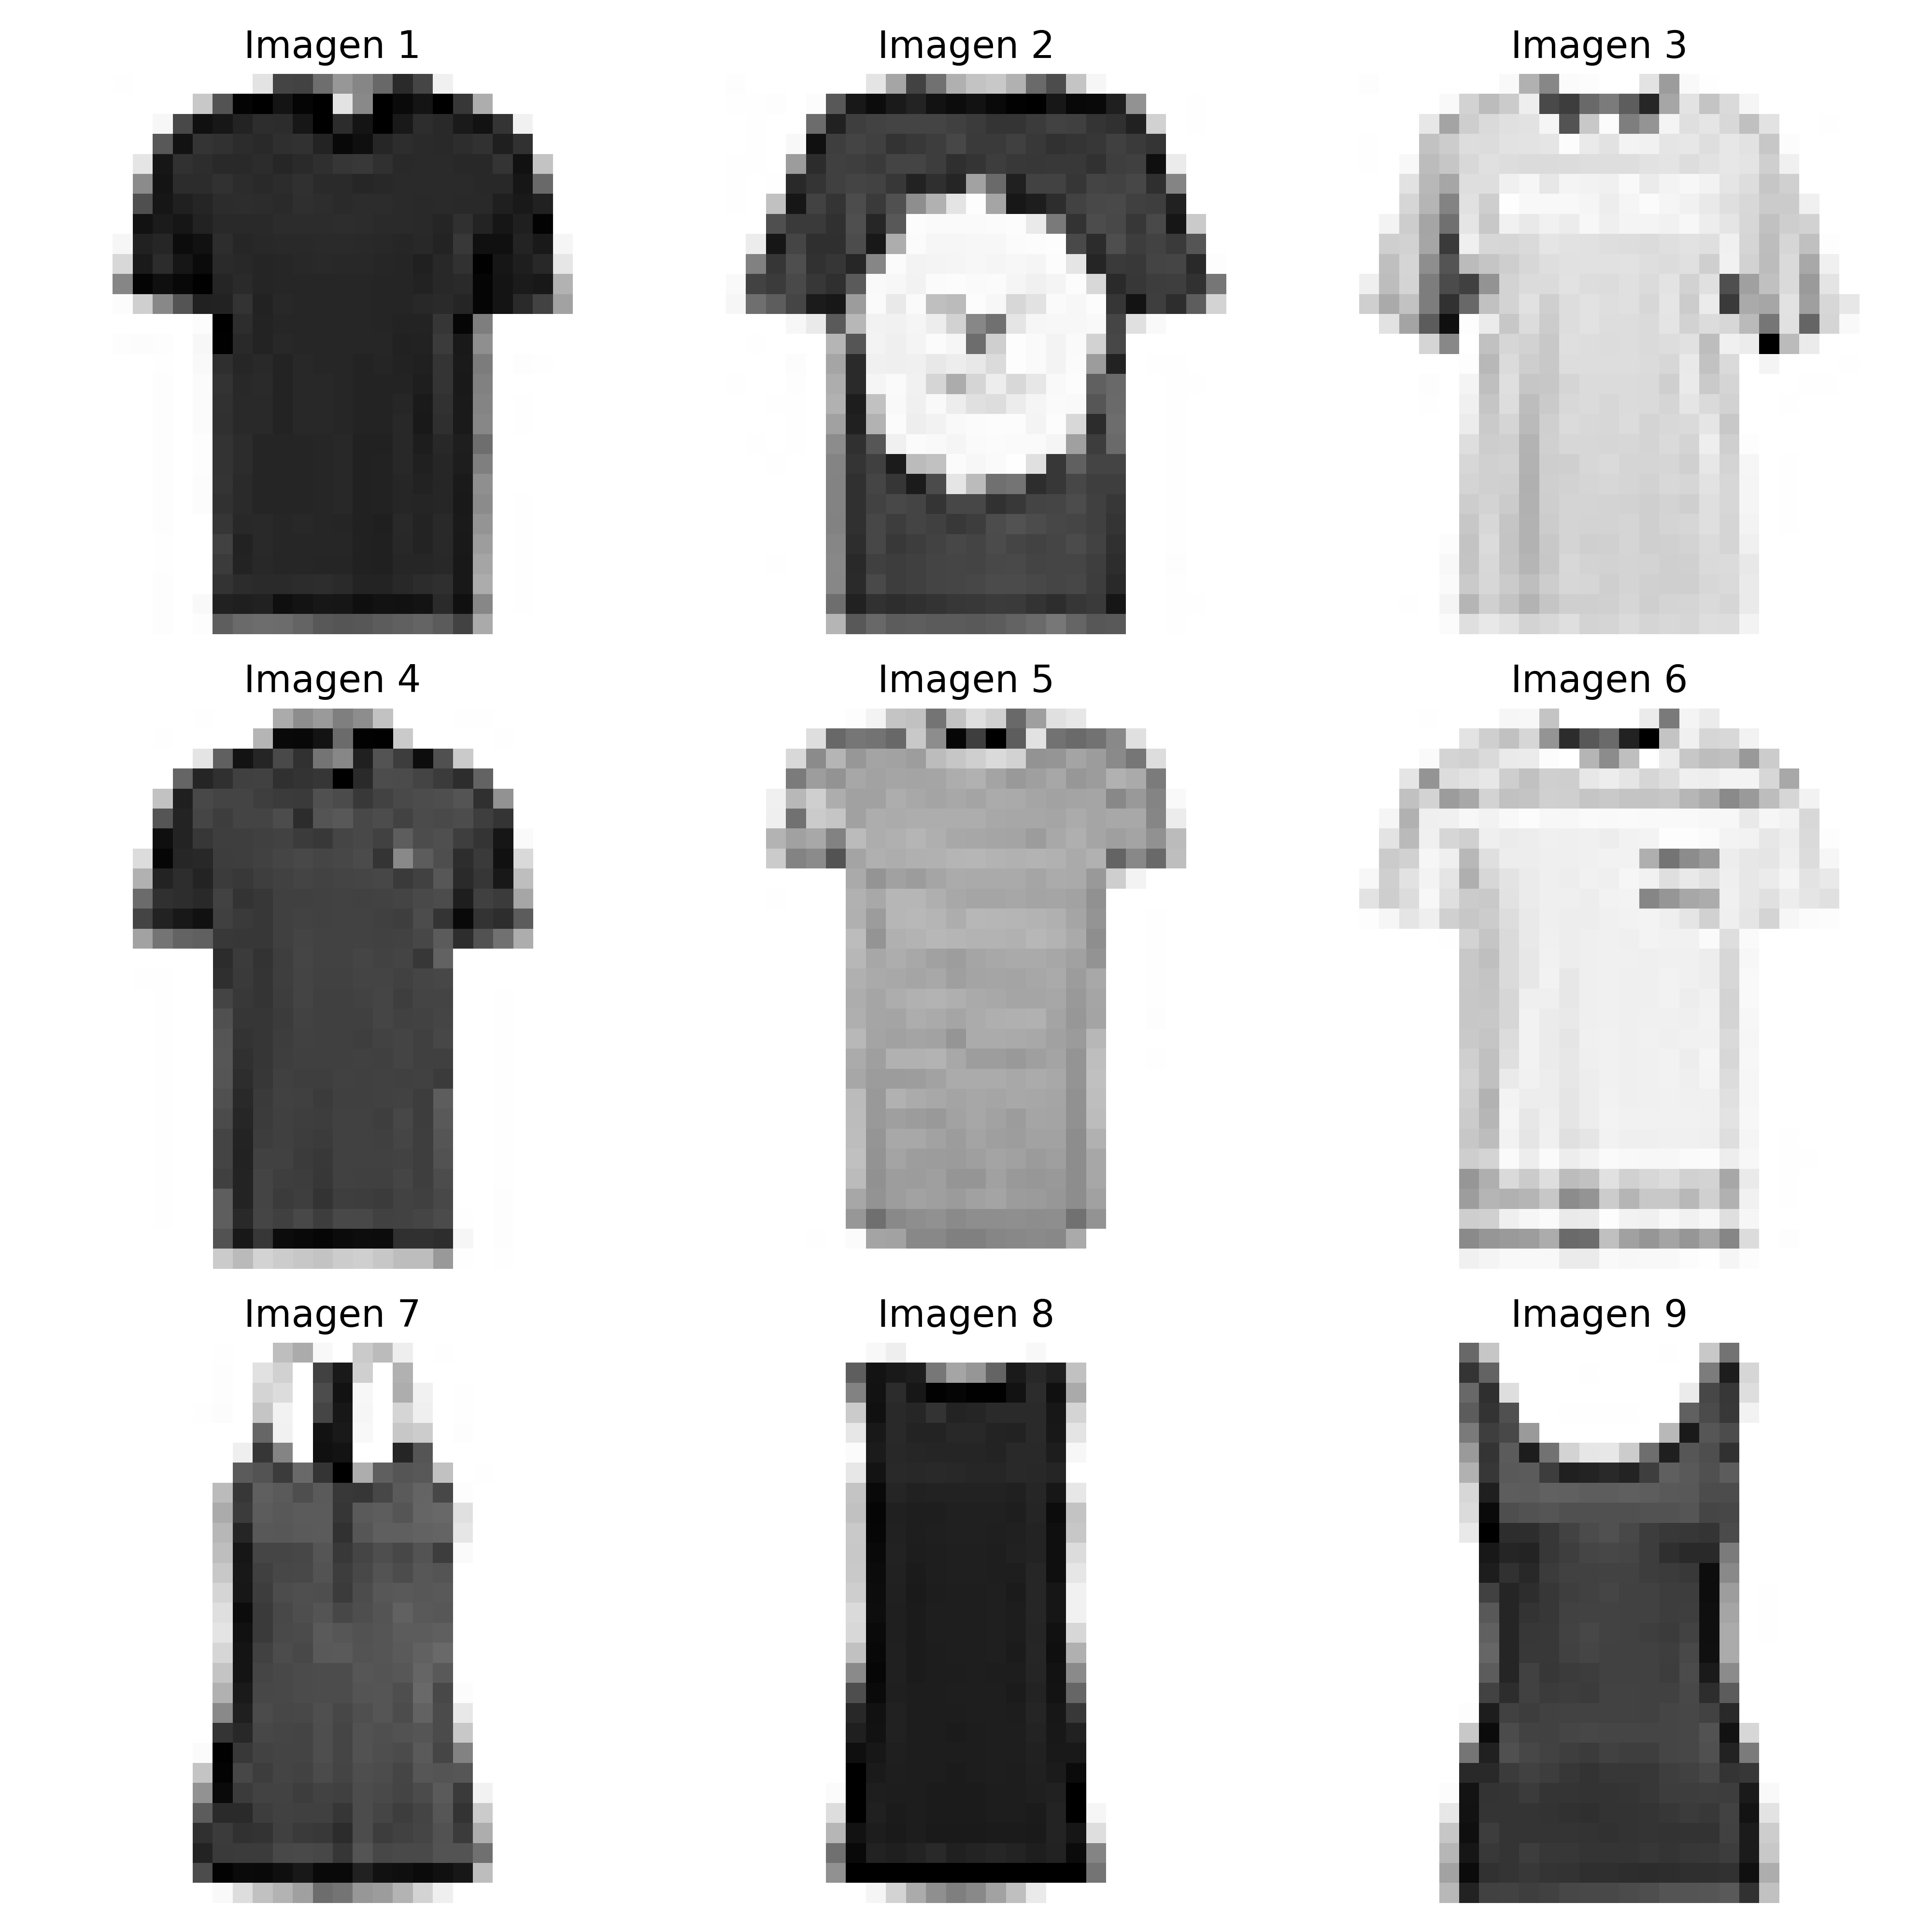
\includegraphics[width=7cm]{Graphics/Problema_3_1/T_shirts_2d.png}
        \caption{}
    \end{subfigure}
    \caption{}
\end{figure}


\begin{table}[H]
    \centering
    \begin{tabular}{ccc} \hline
        \multirow{2}{*}{Imagen} & \multicolumn{2}{c}{Componente}          \\
                                & 1                              & 2      \\ \hline
        1                       & 0.2652                         & 0.6747 \\
        2                       & 0.4111                         & 0.8843 \\
        3                       & 0.6193                         & 0.7453 \\
        4                       & 0.1923                         & 0.3806 \\
        5                       & 0.3552                         & 0.471  \\
        6                       & 0.5223                         & 0.64   \\
        7                       & 0.241                          & 0.011  \\
        8                       & 0.3925                         & 0.1517 \\
        9                       & 0.465                          & 0.3078 \\ \hline
    \end{tabular}
    \caption{}
\end{table}

\subsection*{Visualizaciones 3D}

\begin{figure}[H]
    \centering
    \begin{subfigure}{8.5cm}
        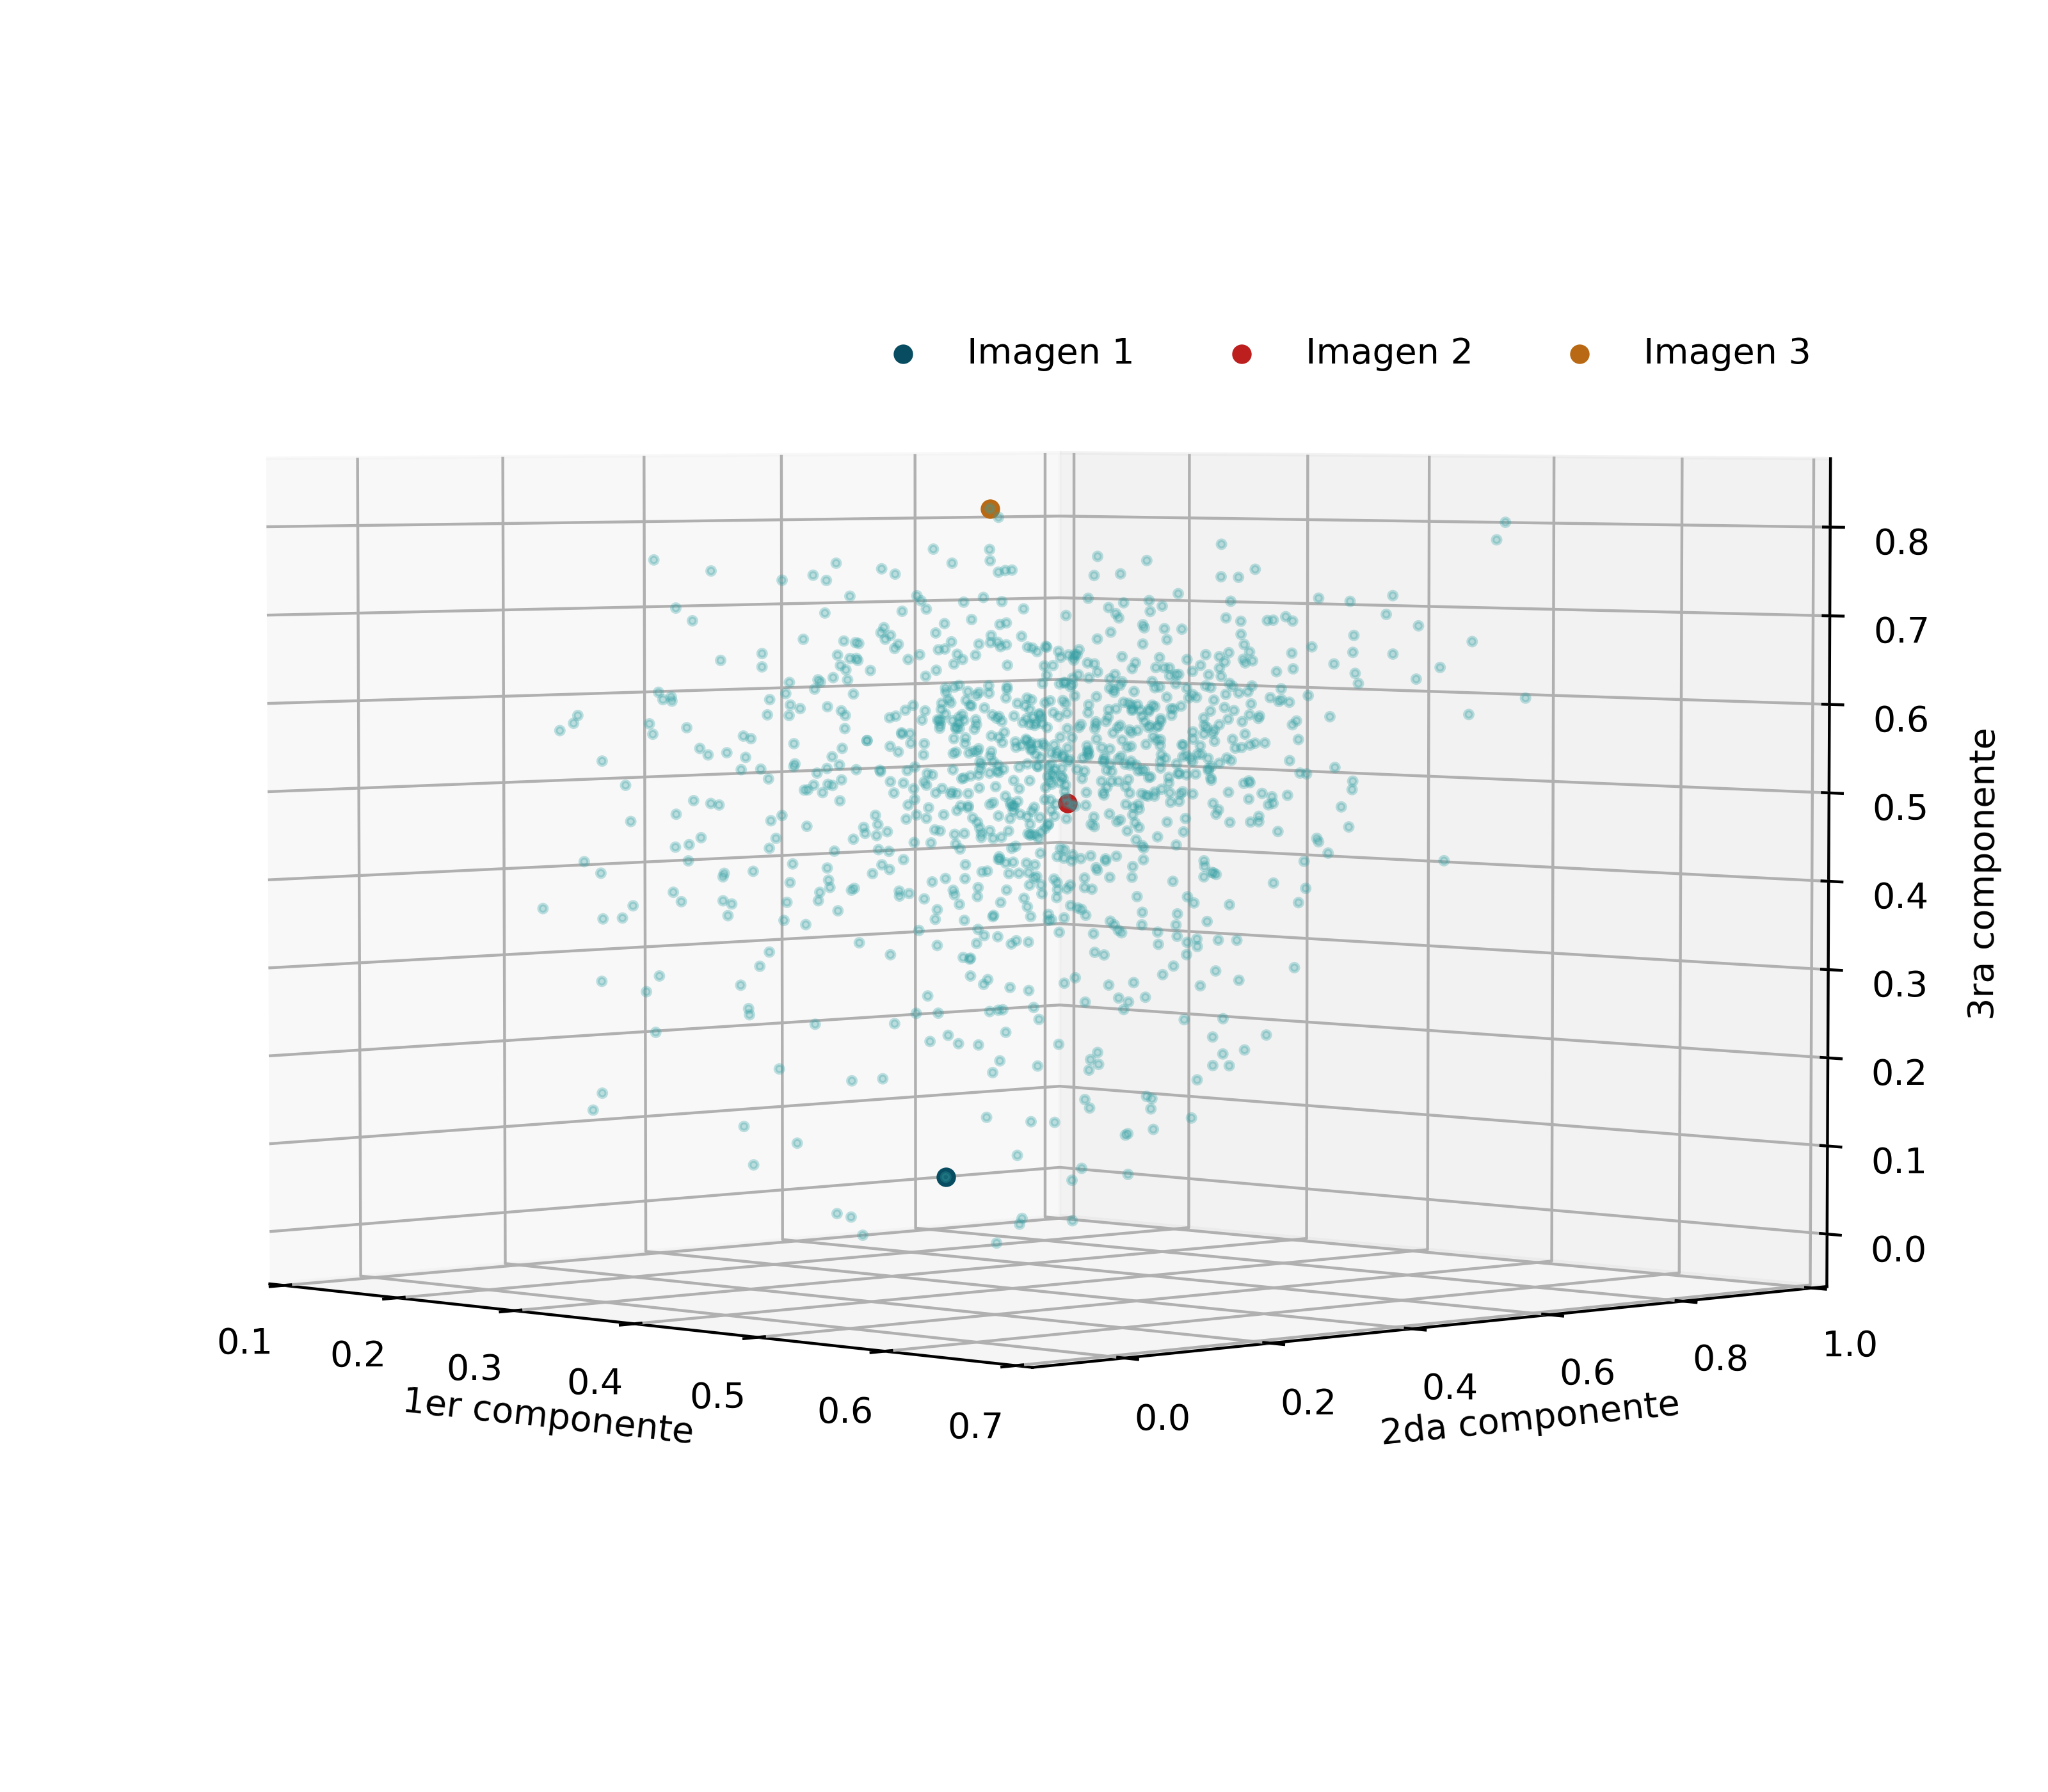
\includegraphics[width=8.5cm]{Graphics/Problema_3_1/loadings_3d.png}
        \caption{}
    \end{subfigure}
    \begin{subfigure}{8cm}
        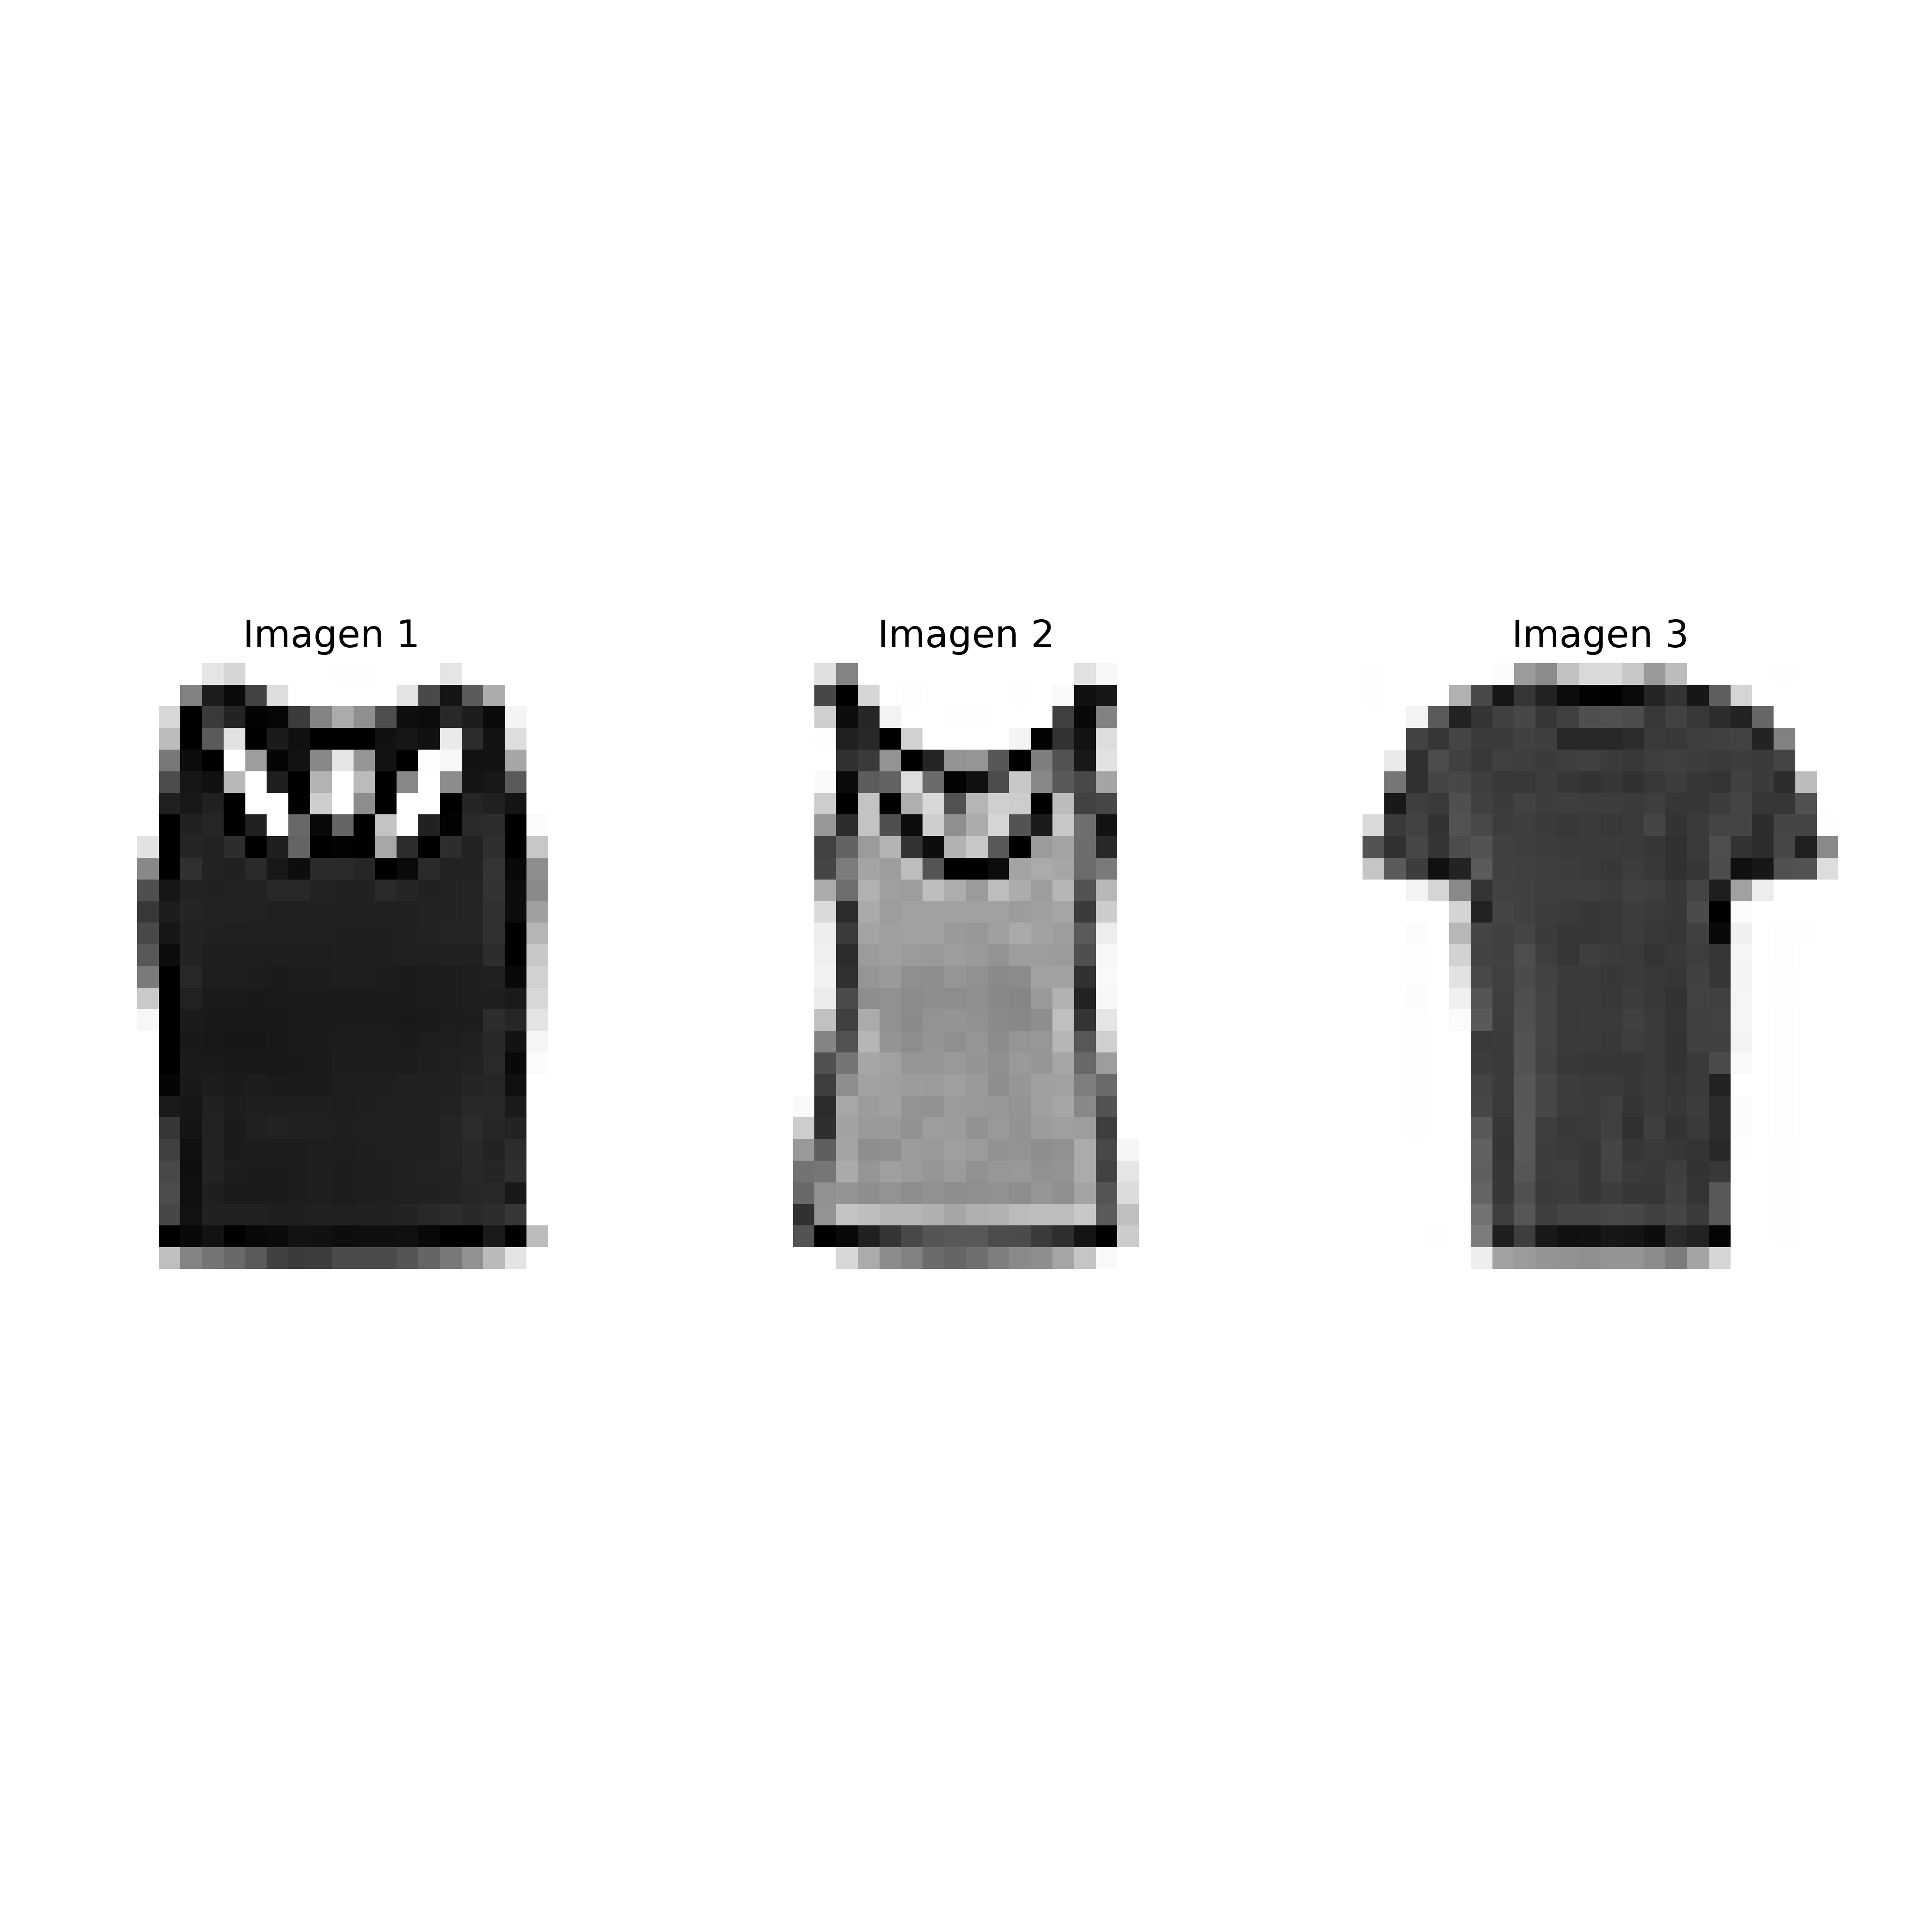
\includegraphics[width=8cm]{Graphics/Problema_3_1/T_shirts_3d.png}
        \caption{}
    \end{subfigure}
    \caption{}
\end{figure}

\begin{table}[H]
    \centering
    \begin{tabular}{cccc} \hline
        \multirow{2}{*}{Imagen} & \multicolumn{3}{c}{Componente}                   \\
                                & 1                              & 2      & 3      \\ \hline
        1                       & 0.3374                         & 0.4134 & 0.058  \\
        2                       & 0.4574                         & 0.377  & 0.494  \\
        3                       & 0.292                          & 0.5571 & 0.8176 \\ \hline
    \end{tabular}
    \caption{}
\end{table}